\section{Experimental Evaluation}\label{sec:eval}

\begin{figure}[t]
  \begin{adjustwidth}{-0.13\textwidth}{-0.13\textwidth}
  	\centering
    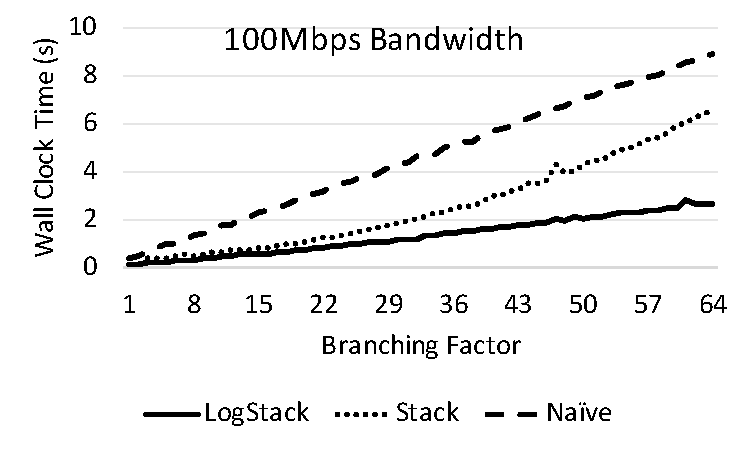
\includegraphics[width=0.4\textwidth]{fig/100mbps}
    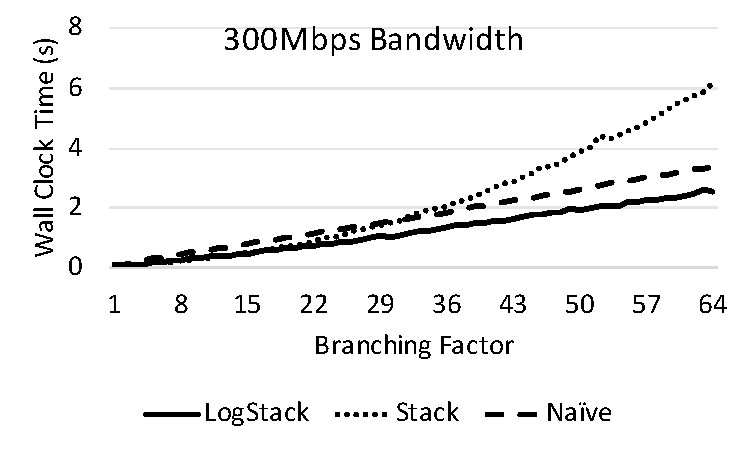
\includegraphics[width=0.4\textwidth]{fig/300mbps}
    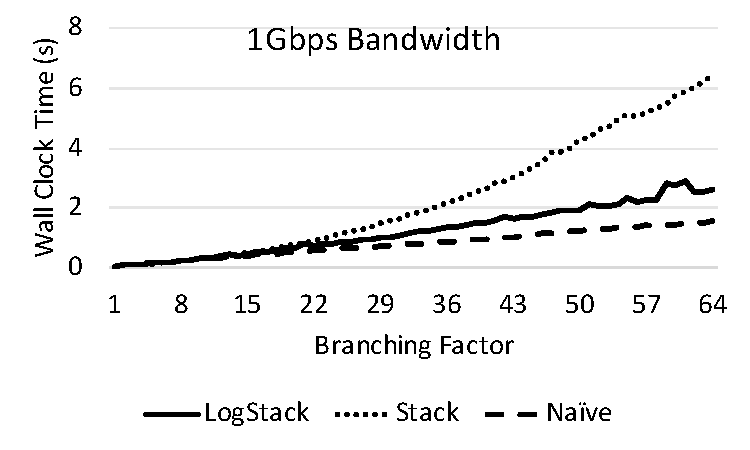
\includegraphics[width=0.4\textwidth]{fig/1gbps}
  	\\
    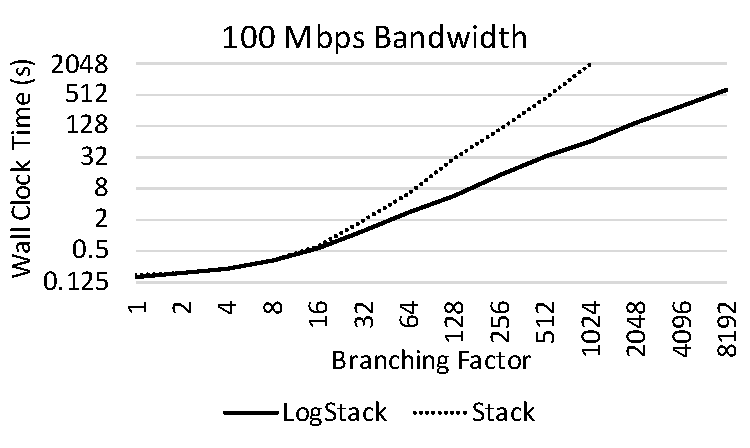
\includegraphics[width=0.4\textwidth]{fig/highbranching}
    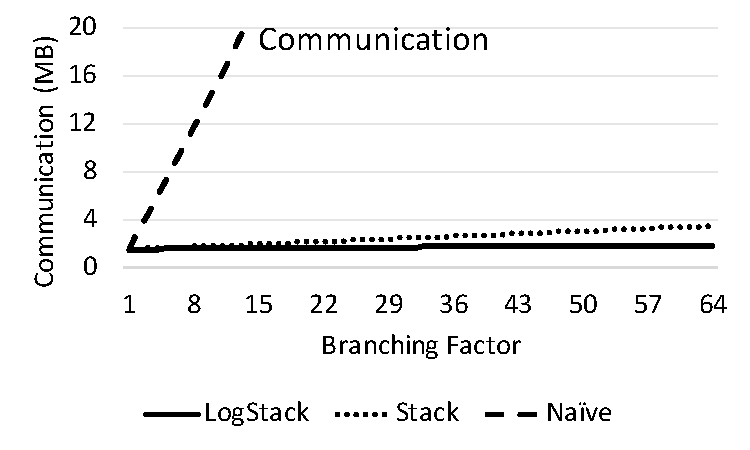
\includegraphics[width=0.4\textwidth]{fig/comm}
    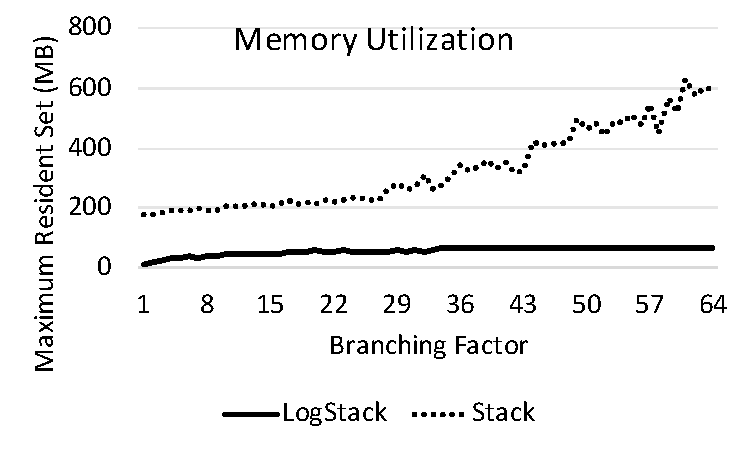
\includegraphics[width=0.4\textwidth]{fig/memutil}
  \end{adjustwidth}
  \caption{%
    Experimental evaluation of \ourschemelong\ as compared to  \HK's
    \stack and to basic half-gates~\cite{EC:ZahRosEva15} (`na\"ive'
    branching).
    We compare in terms of wall-clock time on different simulated network
    bandwidths (top).
    We performed an extended wall-clock time comparison to \stack
    (bottom left).
    Both \ourschemelong\ and \stack\ greatly outperform basic
    half-gates in terms of total bandwidth consumption (bottom
    center), and \ourschemelong\ greatly outperforms \stack\ in terms
    of memory consumption (bottom right).
  }\label{fig:plots}
\end{figure}

We implemented \ourschemelong and extensively experimented with it and
with implementations of basic half-gates~\cite{EC:ZahRosEva15} and the
\stack SGC of~\HK.
Charts in \Cref{fig:plots} plot the results of our experiments.

We consider  the following metrics: end-to-end wall-clock time
performance, bandwidth consumption, and memory utilization.
% of 2PC implemented with each of the three schemes and executed with varying number of branches. 
All branches implement the SHA-256 netlist, which has $47726$ AND gates,
$179584$ XOR gates, and $70666$ NOT gates.
A GC for each branch has size $1.45$ MB.
It is, of course, unrealistic that a conditional would have the same
circuit in each branch. However, we choose this benchmark because
SHA-256 evaluations have become somewhat of a community standard and because our
goal is only to analyze \ourschemelong's performance.
%
We ensure that our implementation does not cheat: it cannot recognize
that the branches are the same and hence cannot shortcut the evaluation.

\paragraph{Total Bandwidth Consumption}  is the easiest metric to analyze.
The communication chart in~\Cref{fig:plots} plots communication
as a function of branching factor.  As expected, \stack's and
\ourschemelong's communication remains almost constant, while half-gates'
grows linearly and immediately dominates.  \ourschemelong is slightly
leaner than \stack because of low-level improvements to
\ourschemelong's demultiplexer. This small improvement should not be counted
as a significant advantage over \stack.

\paragraph{Memory Utilization} was measured as a function of branching
factor.
We compare our scheme to \stack (half-gates memory utilization is
constant, since garblings
can be streamed across the network and immediately discarded).
%
Our chart shows \stack's linear and
\ourschemelong's logarithmic space consumption.
% While \stack uses modest
% space in our experiments, our experiments are on relatively
% small circuits.  For larger branch sizes and more branches, its memory
% consumption may become a bottleneck.  In contrast, our memory
% utilization scales well both with increased branch size and the number
% of branches.
In settings with many branches, improved space consumption
is essential.
For example, we ran \ourschemelong\ on a circuit
with $8192$ SHA-256 branches, a circuit that has $> 385$M
AND gates.  Our peak memory usage was $\sim 100$MB, while \HK
would require more than $12$GB of space to run this experiment.
It would be
infeasible to run this \stack\ experiment on our machine because it
would exhaust our RAM.

\paragraph{Total wall-clock time} to complete an end-to-end 2PC
protocol is our most comprehensive metric.
We plot three charts for 1 to 64
branches (on networks with 100, 300, and 1000 Mbps bandwidth) comparing each of the three approaches.
We also explored more extreme branching factors, running conditionals with
branching factors at every power of $2$ from $2^0$ to $2^{13}$ in the 100Mbps setting.

In the 1Gbps network setting, as expected, na\"ive half-gates leads.
As discussed in~\Cref{sec:whentouse}, two cores (our laptop) indeed
cannot keep up with the available network capacity.  However, doubling
the number of cores would already put us ahead of na\"ive, and any
further computation boost would correspondingly improve
our advantage.  We are about $3\times$ faster than \stack.

In the 300Mbps network setting, we outperform na\"ive.  Because we
range over the same number of branches, we are the same
factor $\approx 3\times$ faster than \stack.

The more typical $100$Mbps setting shows the advantage of SGC.
Both \stack and \ourschemelong handily beat na\"ive.

Finally, we experimented with large branching factors.
\ourschemelong scales well; we ran up to $8192$ branches as it
was sufficient to show a trend.  Due to its logarithmic memory
utilization, \ourschemelong would run on a practically
arbitrary number of branches.  In contrast, \stack exhibited limited
scaling.  We ran up to $1024$ branches with
\stack, enough to show a trend, and after which our experiments
started to take too long.   \ourschemelong ran 2PC for a
$1024$-branch conditional in $\sim 67s$, while \stack took $\sim
2050s$,  $\sim 31\times$ slower than \ourschemelong.


